
\documentclass[tikz,border=5mm]{standalone}
\usepackage{xcolor}

\begin{document}
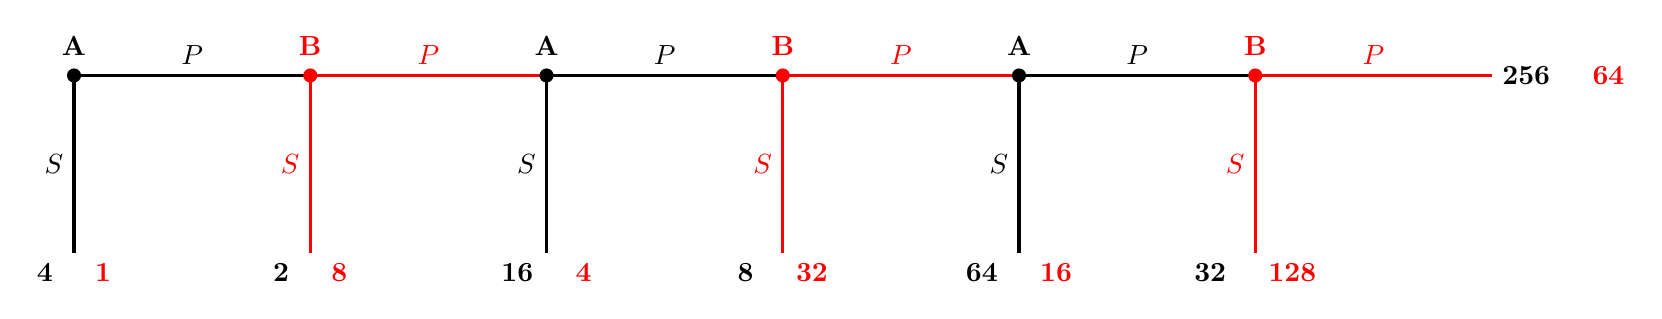
\begin{tikzpicture}[
    scale=1.5,
    font=\bfseries,
    dot/.style={circle, fill=#1, inner sep=1.8pt},
    dot/.default=black,
    line width=1.2pt
]

    % Nodes coordinates
    \coordinate (n1) at (0, 0);
    \coordinate (n2) at (2, 0);
    \coordinate (n3) at (4, 0);
    \coordinate (n4) at (6, 0);
    \coordinate (n5) at (8, 0);
    \coordinate (n6) at (10, 0);
    \coordinate (end) at (12, 0);

    % Downward payoffs coordinates
    \coordinate (d1) at (0, -1.5);
    \coordinate (d2) at (2, -1.5);
    \coordinate (d3) at (4, -1.5);
    \coordinate (d4) at (6, -1.5);
    \coordinate (d5) at (8, -1.5);
    \coordinate (d6) at (10, -1.5);

    % Horizontal branches (Continue / P)
    \draw[black] (n1) -- (n2) node[midway, above] {$P$};
    \draw[red]   (n2) -- (n3) node[midway, above] {$P$};
    \draw[black] (n3) -- (n4) node[midway, above] {$P$};
    \draw[red]   (n4) -- (n5) node[midway, above] {$P$};
    \draw[black] (n5) -- (n6) node[midway, above] {$P$};
    \draw[red]   (n6) -- (end) node[midway, above] {$P$};

    % Downward branches (Stop / S)
    \draw[black] (n1) -- (d1) node[midway, left] {$S$};
    \draw[red]   (n2) -- (d2) node[midway, left] {$S$};
    \draw[black] (n3) -- (d3) node[midway, left] {$S$};
    \draw[red]   (n4) -- (d4) node[midway, left] {$S$};
    \draw[black] (n5) -- (d5) node[midway, left] {$S$};
    \draw[red]   (n6) -- (d6) node[midway, left] {$S$};

    % Decision Nodes & Player Labels
    \node[dot=black, label=above:A] at (n1) {};
    \node[dot=red, label={[red]above:B}] at (n2) {};
    \node[dot=black, label=above:A] at (n3) {};
    \node[dot=red, label={[red]above:B}] at (n4) {};
    \node[dot=black, label=above:A] at (n5) {};
    \node[dot=red, label={[red]above:B}] at (n6) {};

    % Payoffs (A in black, B in red)
    \node[below] at (d1) {4 \quad \textcolor{red}{1}};
    \node[below] at (d2) {2 \quad \textcolor{red}{8}};
    \node[below] at (d3) {16 \quad \textcolor{red}{4}};
    \node[below] at (d4) {8 \quad \textcolor{red}{32}};
    \node[below] at (d5) {64 \quad \textcolor{red}{16}};
    \node[below] at (d6) {32 \quad \textcolor{red}{128}};
    \node[right] at (end) {256 \quad \textcolor{red}{64}};

\end{tikzpicture}
\end{document}

